\documentclass[abstract=on,9pt,twocolumn]{scrartcl}

\usepackage{ucs}
\usepackage[utf8x]{inputenc}
\usepackage[T1]{fontenc}
\usepackage[english]{babel}
\usepackage{datetime}

\usepackage[paper=a4paper,top=2cm,left=1.5cm,right=1.5cm,bottom=2cm,foot=1cm]{geometry}

\usepackage{relsize}%	relative font sizes

\usepackage[retainorgcmds]{IEEEtrantools}%	IEEEeqnarray
\setlength{\IEEEnormaljot}{4\IEEEnormaljot}

\usepackage{graphicx}
\usepackage{epstopdf}
\usepackage{indentfirst}
\usepackage{hyperref}
%\usepackage{cleveref}
\usepackage[noabbrev]{cleveref}
\usepackage{listings}
\usepackage{color}
\usepackage{subfig}

%%%%%%%%%%%%%%%%
%  title page  %
%%%%%%%%%%%%%%%%
\titlehead{University of Minho \hfill Master's Degree in Informatics Engineering\\Department of Informatics \hfill Parallel and Distributed Computing}

\title{Simulated Annealing}

\subtitle{The Room Assignment Problem}

\author{
    \\Miguel Palhas\\
     	\texttt{\smaller pg19808@alunos.uminho.pt}
\and Group 1\\~\\~
\and\\Pedro Costa\\
		\texttt{\smaller pg19830@alunos.uminho.pt}
}

\date{Braga, \docdate}

\subject{Numerical Methods and Algorithms}


%%%%%%%%%%%
%  Hacks  %
%%%%%%%%%%%

%	Paragraph (title) with linebreak
\newcommand{\paragraphh}[1]{\paragraph{#1\hfill}\hfill

}

%	Add "Appendix" to the appendices titles, but not to the references
\usepackage{ifthen}
\newcommand*{\appendixmore}{%
  \renewcommand*{\othersectionlevelsformat}[1]{%
    \ifthenelse{\equal{##1}{section}}{\appendixname~}{}%
    \csname the##1\endcsname\autodot\enskip}
  \renewcommand*{\sectionmarkformat}{%
    \appendixname~\thesection\autodot\enskip}
}

\newdateformat{mmmyyyydate}{\monthname[\THEMONTH] \THEYEAR}
\newcommand{\docdate}{\mmmyyyydate\today}



\begin{document}
	\maketitle
	\begin{abstract}
This document describes the application of the simulated annealing technique to solve the Room Assignment problem and presents a study to prove its effectiveness. Two implementations are presented, a sequential one and a parallel one using MPI. In the parallel implementation, multiple independent processes solve the problem and only the best computed solution is considered. Tests using a manually injected perfect solution proved this technique to improve considerably the results of the basic approach for different numbers of students, specially using multiple parallel processes. Variations in the initial temperature were proven to affect mainly the convergence of the method.
\end{abstract}

	\section{Introduction}
%	Contextualização
Physical annealing is a process through which a melted metal is allowed to cool slowly, thus forming a defect-free crystal with a regular structure. At higher temperatures the atoms move more freely and rearrange their structure easily. As the temperature decreases, the ability for the atoms to move is diminished since they possess less energy. This allows the material to reach a state of minimum energy -- the crystalline form.

Simulated annealing is an iterative method based on the process of physical annealing for solving combinatorial optimization problems. The system starts at a given (high) temperature, which allows the algorithm to choose and follow a worse solution according to a probability function based on the temperature. In each iteration, a cooling function decreases the system temperature, also decreasing the probability for a worse solution to be followed. Without simulated annealing, the algorithm never accepts a worse solution, which causes it to be trapped in local solutions. With simulated annealing, the algorithm is allowed to change the system state from a local solution to a worse state, which eventually leads to a state closer to the global solution.

%	Motivação
This document aims to study the impact of the simulated annealing method in an usual use case (the room assignment problem) and how the solutions obtained react to the variation of the parameters.

%	Objectivos
In this project two versions are implemented to solve this problem: the first being the sequential implementation and the second being a parallel implementation using MPI. Both versions implement two approaches, one using a strictly minimizing method and another using the simulated annealing method. For each version, both approaches are tested using the same matrix of incompatibility values for a range of different numbers of students to be assigned. The simulated annealing approach is also tested using different initial temperature values.
	\section{The Room Assignment Problem}
\label{sec:problem}

The room assignment problem is a combinatorial optimization problem where the simulated annealing method allows better solutions to be achieved.

The problem consists in assigning $n$ students to $\frac{n}{2}$ rooms, but in a way that minimizes the probability of a conflict occurring. The chances for such conflicts to occur are measured in a matrix $D$ of $n^{2}$ integer values, where each element $d_{i,j} = d_{j,i}$ represents how much students $i$ and $j$ dislike each other. In any iteration, the current system state is represented by a vector $S$ of $\frac{n}{2}$ pairs of elements, where each pair $(i,j)$ represents the two students assigned to a room\footnote{Since $d_{i,j}=d_{j,i}$ then $(i,j)\in S\Leftrightarrow(j,i)\in S$. In other words, the order within the pair is neglected.}. The total cost of a state $S$ is given by the sum of all the $d_{i,j}$, where $(i,j)\in S$. A formal definition of this problem as an optimization problem is presented in \cref{fig:formaldef}.

\begin{figure}
	\begin{center}
		\fbox{
		\parbox{0.9\columnwidth}{
			\paragraph{Decision Variables}
			\begin{itemize}
				\item{$d_{i,j}$ --- level of incompatibility between the students $i$ and $j$;}
			\end{itemize}
			
			\paragraph{Decision Restrictions}
			\begin{itemize}
				\item{$0 \leq i \leq n$}
				\item{$0 \leq j \leq n$}
				\item{$\forall i,j : 0 \leq d_{i,j} \leq 10$}
			\end{itemize}
			
			\paragraph{Objective Function}
			\begin{IEEEeqnarray}{lCr}
				\mathrm{min}\;:\;\mathbf{Cost}(S) & = & \sum\left\{d_{i,j}:(i,j)\in S\right\}
			\end{IEEEeqnarray}
		}
		}
	\end{center}
	\caption{Formal definition of the Room Assignment Problem as an optimization problem.}
	\label{fig:formaldef}
\end{figure}

The goal in this problem is to find a state for which the cost is minimized. However, for $n$ students there are $(n-1)\times (n-3)\times\ldots\times 3$ possible distributions -- this has the order of magnitude of $\sqrt{n!}$, which makes it unfeasible to analyze every single possible state. Alternatively, with an heuristic method, while it does not guarantee the optimal solution, it allows to calculate a good approximation with significantly less effort.

The heuristic approach to this problem starts by generating a random room distribution. In each iteration, two students in distinct rooms are randomly selected and swapped. If the new state has a lower cost, the change is accepted, otherwise it is reversed.

The simulated annealing method changes how the decision about accepting or refusing the swap is taken. With no simulated annealing, only a state with lower cost is accepted. This causes the system to be trapped in local minimum. With simulated annealing, the system is initialized at a given (high) temperature and a higher cost state is accepted with probability $e^{-\Delta/T}$, where $\Delta$ is the difference between the cost of the two states (before and after the swap). A cooling function is used in each iteration to (slowly) decrease the temperature.
	\section{Implementation}
\label{sec:implementation}
The program implemented to solve the Roommate Assignment problem uses both approaches -- with and without simulated annealing -- with the same generated incompatibility matrix. The problem is solved by a function named \texttt{distribute} that is included at two distinct points of the code with different preprocessor environments. This benefits debugging by reusing the common code of both approaches.

The number of students -- $n$ -- and the initial temperature -- $T_{0}$ -- are given as arguments. $n$ is used to allocate the global incompatibility matrix ($n^{2}$) and the room distribution vector ($n$), which is used by the \texttt{distribute} function to output the result. The program then proceeds in generating the values for the incompatibility matrix, and injects a perfect solution.

The \texttt{distribute} function starts by allocating an auxiliary vector, which is used to track the room assigned to each student (in contrast with the output vector that tracks the students assigned to each room). An initial student distribution is then randomly generated, and the current state cost is calculated. In the simulated annealing approach, the temperature is set to the given initial value at the end of this stage.

The iterative process to find a solution in the \texttt{distribute} function is limited by the number of stagnant iterations ($n^{2}$). In each iteration, two students in distinct rooms are randomly selected\footnote{Both rooms and students are identified by integer non-negative numbers. The former correspond to an index in the output vector, the latter to an index in the auxiliary vector.} and the cost of swapping them is calculated. If the cost of the swap is less than the current cost -- or, with simulated annealing, if the temperature is high enough for $e^{-\Delta/T}$ to exceed a randomly generated value -- the swap is accepted and the stagnant iterations counter is reset; otherwise, the state is not modified and the counter is incremented. With simulated annealing, the temperature is reduced at the end of each iteration using the cooling function $T_{i+1}=0.999\times T_{i}$.

One of the key points in this algorithm is precisely the condition of acceptance based on the \texttt{exp} function. This condition, meant to decide whether a worse state will be accepted or not, always causes a state with equal cost to be accepted. Despite not changing the cost, rearranging some students may unlock better combinations in the next iterations, which makes this a desirable feature. At the same time, in late stages of the execution, when the temperature is so low that only the better solutions are accepted, this may cause the algorithm to follow loops, constantly resetting the stagnant counter and extending the execution time beyond usable walltimes. To correct this, a second iteration counter is added, which is reset only when the cost is changed. While this new counter allows the algorithm to keep accepting states with the same cost, it forces the stop when too many iterations have passed with no improvements.

\subsection{Parallelism}
\label{sec:parallelism}
The algorithm used to solve the Room Assignment problem is embarrassingly parallel: if each process calculates a different solution using a different sequence of pseudo-random numbers, multiple processes are more likely to get closer to the perfect solution using the same stagnant iterations threshold.

The parallel version of this program was implemented using a \textit{Message Passing Interface} (MPI) library. After the proper library initialization, the root process reads the values for $n$ and $T_{0}$, and broadcasts them to every other process. Each process then proceeds to allocate the necessary memory for the incompatibility matrix. The root process then generates the matrix values and broadcasts it to every other process. The room distribution vector is allocated by each process, and all solve the problem independently of the rest. In the end, a reduction to find the minimum cost is performed for each approach, and the root process outputs those values as the final results.
	\section{Experimental Comparison}
\label{sec:comparison}

\subsection{Environmental Setup}
\label{sec:environment}
All the tests were meant to performed in the SeARCH cluster\footnote{\texttt{http://search.di.uminho.pt}} using a specific group of computational nodes, referred in this document as SeARCH Group Hex. Yet, due to problems in using this cluster, most tests ended up being tested in a MacBook Pro laptop.

SeARCH Group Hex contains twelve nodes, each with two hex-core processors (with Intel{\textsuperscript{\textregistered}} Hyper-Threading Technology) and up to 48 GB of RAM. The detailed hardware description for the nodes in this group is presented in \cref{tab:grouphex}.

\begin{table}[!htp]
	\begin{center}
		\begin{tabular}{ll}
			\hline
			Processors per node: & 2	\\
			Processor model: & Intel{\textsuperscript{\textregistered}} Xeon{\textsuperscript{\textregistered}} X5650\\
			Cores per processor: & 6	\\
			Threads per core: & 2	\\
			Clock frequency: & 2.66 GHz	\\
			\hline
			L1 cache: & 32 KB + 32 KB per core	\\
			L2 cache: & 256 KB per core	\\
			L3 cache: & 12 MB shared	\\
			RAM: & 12 to 48 GB	\\
			\hline
		\end{tabular}
		\caption[SeARCH Group Hex hardware description]{SeARCH Group Hex hardware description. See \cite{xeon5600} for further detail about this processor.}
		\label{tab:grouphex}
	\end{center}
\end{table}

The MacBook Pro laptop used for the tests is a mid-2010 model with one dual-core processor (with Intel{\textsuperscript{\textregistered}} Hyper-Threading Technology) and 4GB of RAM. The detailed hardware description for this laptop is present in \cref{tab:mbp}.

\begin{table}[!htp]
	\begin{center}
		\begin{tabular}{ll}
			\hline
			Processors: & 1	\\
			Processor model: & Intel{\textsuperscript{\textregistered}} Core{\textsuperscript{\texttrademark}} i5-520M\\
			Cores per processor: & 2	\\
			Threads per core: & 2	\\
			Clock frequency: & 2.40 GHz	\\
			\hline
			L1 cache: & 32 KB + 32 KB per core	\\
			L2 cache: & 256 KB per core	\\
			L3 cache: & 3 MB shared	\\
			RAM: & 4 GB	@ 1067 MHz (DDR3)\\
			\hline
		\end{tabular}
		\caption[MacBook Pro mid-2010 hardware description]{MacBook Pro mid-2010 hardware description. See \cite{i5-520m} for further detail about this processor.}
		\label{tab:mbp}
	\end{center}
\end{table}

\subsection{Methodology}
\label{sec:methodology}

The two versions of the implementation described in this document were measured separately with the same methodology. Both were measured for different values of $n$ from 40 to 200 with a step of 4. The approach with simulated annealing was tested using $T_{0}=1$, $T_{0}=10$ and $T_{0}=10^{4}$. Larger values of $n$ were intended, but due to problems in using the SeARCH cluster and execution time constraints, such tests could not be completed.

For each pair $(n,T_{0})$, 10 executions were performed. When comparing the final solution cost, the accepted resulting value is the minimum value of all executions. For comparing numbers of iterations, the average of all executions is accepted as result.

The distributed memory version was also tested using different numbers of processes. Tests up to 16 processes were performed in the MacBook laptop. Any test larger than that was performed using SeARCH Group Hex nodes.

When relevant, cost related tests were also performed using two different \textit{Pseudo-Random Number Generators} (PRNG): the classic \texttt{rand} generator, present in the C standard library, but often described as a very weak generator; and the \texttt{arc4} generator, present in the BSD library, often described as the best alternative for \texttt{rand}. The \texttt{arc4} generator is not available in the SeARCH cluster.

\subsection{Results}
\label{sec:results}

\begin{figure}
	\begin{center}
		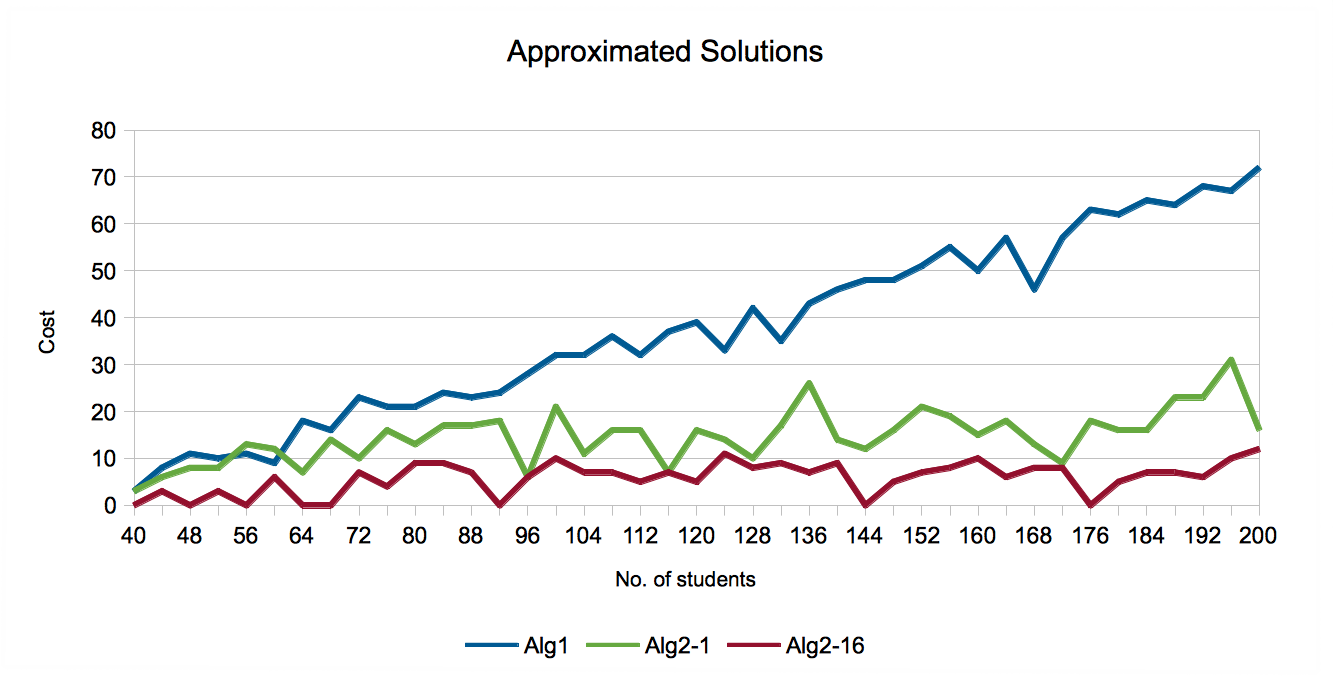
\includegraphics{report/images/t0-01.png}
		\includegraphics{report/images/t0-10.png}
	\end{center}
\end{figure}
	\section{Conclusion}
\label{sec:conclusion}

	\bibliographystyle{cell}
	\bibliography{references}

\end{document}
